\section{Contribution 1: Swarm Control}

\subsection{Introduction}
In this section, we present our first contribution, which is the drone control kernel. We present the software architecture that we have developed to control drones in a swarm. We also present the results of the evaluation of the drone control kernel.


We were provided a synchronous control driven \gls{API} we have worked around it to handle practial asynchronous calls. We show here this work.


\subsection{Drone Control Kernel}

\subsubsection{Introduction, Motivation and Objectives}
Currently, Crazyflie drones are controlled using their Python library, cflib, which provides developers with a robust toolkit for sending commands, receiving sensor data, and managing flight tasks. While this library offers powerful capabilities, it limits the flexibility of using the Python ecosystem, as direct access to the drones requires interacting through this specific interface. As a result, broader accessibility for developers or users unfamiliar with Python is restricted, making it challenging for people from diverse technical backgrounds to engage with drone control.

To address this limitation and open drone control to a wider audience, we propose a web-based control platform. By developing a web interface, we aim to abstract the complexities of the underlying Python-based system and make the control of drone swarms more accessible to a larger range of developers, including those familiar with other technologies. This approach democratizes drone control, allowing users to interact with Crazyflie drones through web-based \gls{API}s and interfaces, facilitating easier integration into various applications, including human-drone interactions in indoor environments.

Instantaneous \gls{API} Calls and Background Processing: Asynchronous \gls{API}s enhance the functionality of drone control applications by handling requests in the background. This approach maintains application functionality while keeping resources free to process new requests. Especially in drone operations where real-time responsiveness is crucial, this capability ensures efficient handling of multiple tasks simultaneously.

Adaptability to Connectivity and Execution Time: Asynchronous \gls{API}s are particularly beneficial in environments with variable connectivity or where requests have longer execution times. They allow for the processing of complex operations without causing delays in the application's responsiveness, crucial for real-time drone control where delay can have significant consequences.

Event-Driven Communication: Asynchronous \gls{API}s, enable more intelligent communication between internal and external services. This is especially important in drone operations where multiple events or commands may need to be handled in real time, ensuring smoother and more efficient workflows

Support for Various Protocols: These \gls{API}s support a range of messaging protocols and transports such as WebSockets and UDP subscriptions, which are essential for the dynamic and varied requirements of drone control. This flexibility allows for fast and more accessible and versatile drone operation management.
\subsubsection{Heritage and Components Used in the Project}
The drone control kernel consists of several components that work together to provide a robust and flexible control system for managing drone swarms. Crazyflie drones being used in this project communicate using the Radio component Crazy Radio PA. We include also decks that can be added to the drones to add the location of the drones using light house technology. This requires a specific deck to be added to the drones and lighthouses to be placed around the room. The drones are then able to locate themselves in the room.
\cite{carstens_intelligent_nodate}

\subsubsection{Theory}
According to the state of the art the drones can be controlled using different localization methods. The lab's legacy left us the Lighthouse positioning system. This system uses infrared light to locate the drones in space. The drones have a deck that can be added to them to allow them to locate themselves in space.

\begin{figure}[htbp]
    \centerline{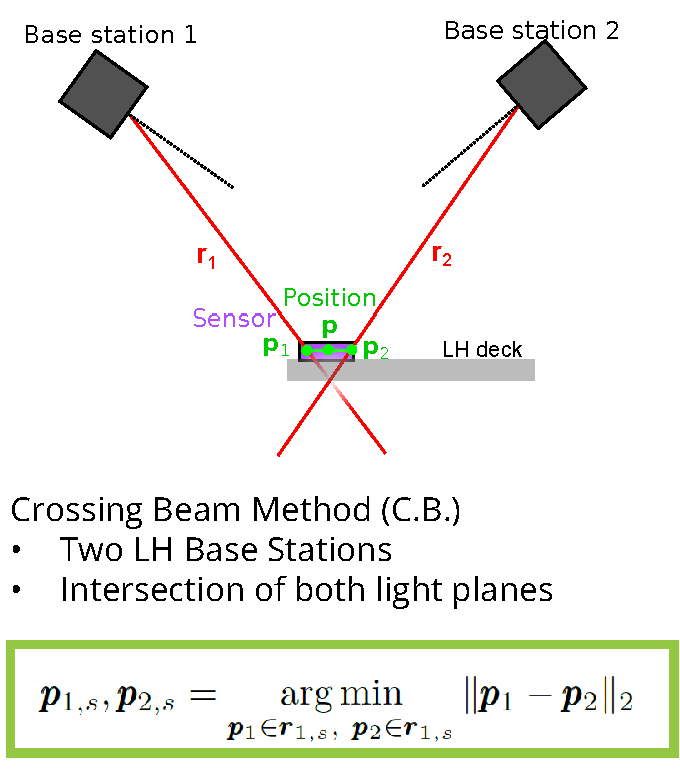
\includegraphics{images/lighthouseworking.png}}
    \caption{Drone Control Kernel, showing the workings of the Lighthouse positioning system.The idea is to calculate the vectors from two base station to a sensor on the Lighthouse deck. This vector is defined by the intersection line between the two light planes of the base station and is sometimes referred to as a “beam”, hence the name.
    In theory the beams should cross in the point where the sensor is located. In reality the point that is closest to both beams is used instead, and uses this as the estimated position. \cite{noauthor_lighthouse_nodate}}
    \label{fig}
    \end{figure}

\subsubsection{Components Evaluation}

We have evaluated the components of the drone control kernel to ensure that they meet the requirements of the system. The results of the evaluation are presented in the following sections.

We expected the drones to follow a smooth path and found that the drones were able to follow the path with a high degree of accuracy. The drones were able to maintain their position and orientation while moving along the path, demonstrating the effectiveness of the control system. 
\begin{figure}[htbp]
    \centerline{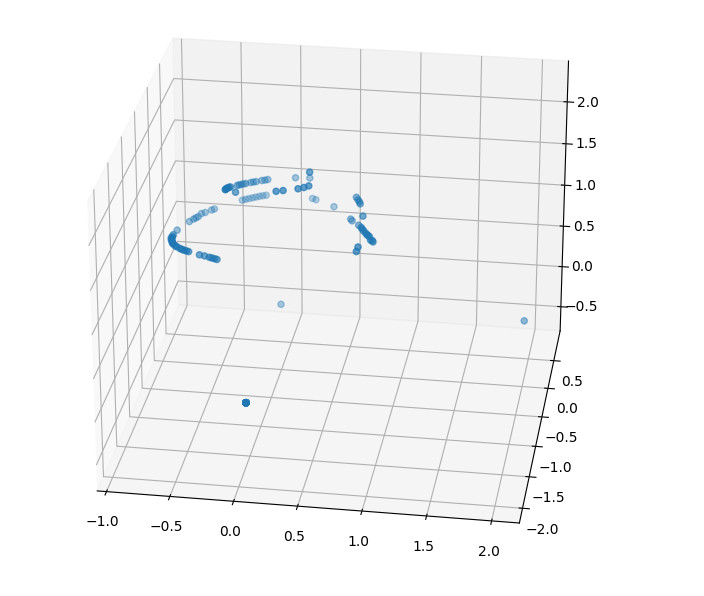
\includegraphics{images/pos.jpg}}
    \caption{Drone Components evaluation.}
    \label{fig}
    \end{figure}


\subsubsection{Architecture}
The drone control kernel is designed to provide a robust and flexible control system for managing drone swarms. The architecture of the drone control kernel is shown in Figure 1. The main components of the system are: 
Web \gls{API}, which provides the web-based interface for controlling the drones; 
Socket, which allows for lower level client drone server interface with the drones; and the Drone Control Kernel, which manages the communication with the drones using Radio. 
The UDP server runs in parallel with the Fast\gls{API} application, thanks to $asyncio.create\_task()$. \cite{asyncio} This allows the UDP server to handle datagram messages asynchronously while the FastAPI server responds to HTTP requests.

\begin{figure}[htbp]
    \centerline{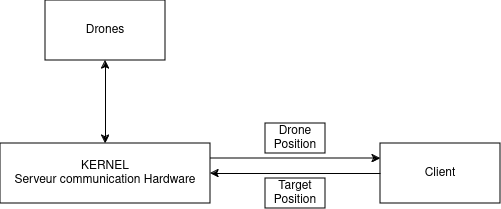
\includegraphics{images/DronecontrolKernel.png}}
    \caption{Drone Control Kernel, showing the main components of the system.}
    \label{fig}
    \end{figure}

\begin{figure}[htbp]
    \centerline{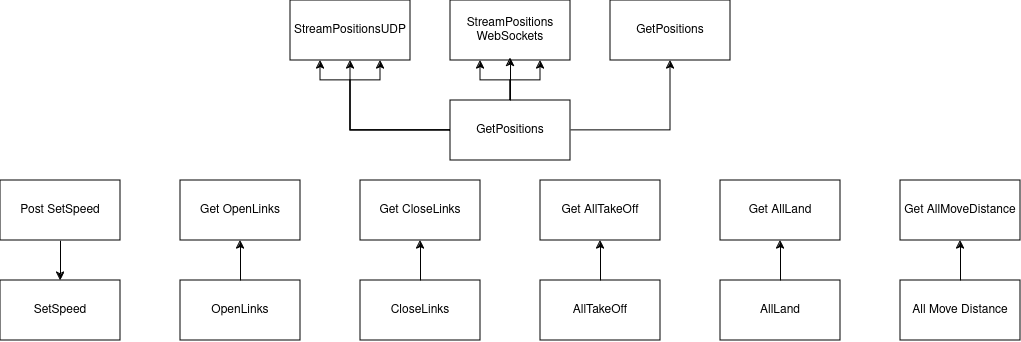
\includegraphics{images/DroneLogics.png}}
    \caption{Drone Control Kernel, inside logics.}
    \label{fig}
    \end{figure}
Using FastAPI we are able to provide a basic web based interface to control the drones. The UDP Client is used to get positions of the drones without having to wait for the drones to respond or the client to send an Acknowledgment. It is used to lower the latency of the system and to stop the package drops errors given by the TCP server on load.



Each function in the UDP server is a coroutine, which allows for asynchronous execution. The UDP server listens for incoming messages from the drones and processes them accordingly. The FastAPI application provides the web-based interface for controlling the drones. It exposes various endpoints for sending commands to the drones, such as takeoff, land, and move. The FastAPI application communicates with the UDP server to send commands to the drones and receive responses. The Socket component provides a lower-level interface for communicating with the drones using the Crazyflie Python library. It handles the connection to the drones and sends commands to them using the cflib \gls{API}. The Drone Control Kernel manages the communication with the drones using the Radio. It sends commands to the drones and receives responses from them using the Radio component (Crazy Radio PA).

Also a ThreeJS interface is provided to visualize the drones in \gls{3D} space. This interface allows users to see the drones' positions and orientations in real-time, providing a visual representation of the swarm's behavior. The ThreeJS interface communicates with the FastAPI application to receive updates on the drones' positions and orientations.
\subsection{Evaluation and Results}

We have realized that the drone control kernel had a big flaw using TCP based technologies as we would observe drops in the communication. We have then switched to UDP based technologies and have seen a big improvement in the communication. We have also seen that the drones were able to follow a path with a high degree of accuracy. The drones were able to maintain their position and orientation while moving along the path, demonstrating the effectiveness of the control system.
We werent able to break this server as we were able to send 1000 requests per second to the server and the server was able to handle them all as no function blocks the system.
This was possible because the server was made as stateless as possible. So after setup no command could break it.

There is also a big improvement in the latency of getposition requests. The TCP server would take between 0.2 and 0.5 seconds to respond to a getposition request. The UDP server is able to respond in less than 0.05 seconds using cflib low level variable accessibility. This is a big improvement in the latency of the system.
\subsection{Conclusion}

Using the drone control kernel, we have developed a robust and flexible control system for managing drone swarms. The system provides a web-based interface for controlling the drones and visualizing their positions and orientations in real-time. The system is designed to be scalable and extensible, allowing for the addition of new features and functionalities as needed. The system has been evaluated and shown to be effective in controlling drones in a swarm, with the drones able to follow a path with a high degree of accuracy using the Lighthouse positioning system. The system provides a valuable tool for developers and researchers working with drone swarms, enabling them to experiment with different control strategies and algorithms.
